\documentclass[12pt,letter]{article}
\usepackage{amssymb,microtype,tikz, amsmath, hyperref,setspace,todonotes}
\usepackage[T1]{fontenc}
\usepackage{color,parskip,siunitx,physics,marginnote}
\DeclareMathAlphabet{\mathscr}{OT1}{pzc}{m}{it}
\usepackage{epsfig, graphicx,subcaption,caption}
\usepackage{verbatim,marginfix}
\captionsetup[widefigure]{size = \textwidth}
\renewcommand{\footnotesize}{\scriptsize}
%\usepackage{mparhack}
\usepackage[driver=xetex,inner=2cm, outer=6cm, marginparsep=.5cm, marginparwidth=5cm, 
twoside=true]{geometry}
\usepackage[maxfloats=45]{morefloats}
\newcommand{\marginparstyle}{\footnotesize} % initialize style with start value
  \renewcommand*{\marginfont}{\marginparstyle}
\let\oldmarginpar\marginpar
\renewcommand*{\marginpar}[1]{\oldmarginpar{\begin{singlespace*} \marginparstyle #1
\end{singlespace*}}}
\usetikzlibrary{shapes.geometric, arrows}
\usepackage{ebgaramond,sidenotes}
\title{Laser-Wakefield Electron Accelerators}
\author{Adam A. S. Green}
\begin{document}
\bibliographystyle{plain}
\maketitle
\doublespacing
\strictpagecheck

\begin{abstract}
In the late 1970's, Tajima and Dawson proposed a method of acceleration 
electron using the large electric field gradients that plasmas are capable of 
sustaining. They showed that when a large amplitude laser pulse is sent through 
an plasma, it is capable of creating a co-propogating longitudinal plasma wave 
that is capable of having an electric field gradient of multiple Gev/cm-- orders
of magnitude larger than that of conventional particle accelerators.. 

In this work, we review the state-of-the-art experimental progress being made 
in creating a fully functioning electron accelerator based on laser plasma 
acceleration (LPA) technology. We discuss how the energy in a  transverse, 
oscillitory electric field of a high intensity pulsed laser can be converted 
into an electric field gradient that can be used to accelerate electrons, and 
we will briefly review the physics of its propogation.  \end{abstract}
\tableofcontents
\section{Introduction}
\label{sec:intro}
Laser plasma wakefield accelerators (LPWA) will be a revolutionary technology
for scientists. The acceleration gradients that plasmas are capable of
sustaining are many orders of magnitude larger than conventional particle
accelerators. This allows technologies based on plasmas, such as LPWA, to be
orders of magnitude smaller.
 Much like the introduction of the personal computer in the era of massive
 supercomputers, LPWA will put the technology of electron acceleration to
 large\sidenote{Multiple GeV's} energies in the hands of many.
 The ability to accelerate particles to high energies is a cornerstone
 in many areas of science. Although the recent discovery of the Higgs
 boson\cite{} at the LHC demonstrated the value of ion-accelerators capable of
 TeV energies, a more direct comparison to the regimes acheivable to LPWA
 technology would be to linacs-- such as Stanford Linear Accelerator Center
 (SLAC), which can accelerate electrons to hundreds of GeVs\cite{}.

 Although historically important to the development of particle
 physics\footnote{The experimental discoveries of the quark, and the tau lepton
 were made at SLAC}, the most broad application of linacs such as SLAC is the use of
 accelerated electrons for an free-electron x-ray laser; the development of
 which has allowed investigation of structures from biology to solid state
 physics, as well as pioneering techniques in medical imaging.\cite{}
 

 But, much like the supercomputers of the 80's, the future of the field is limited by the size and expense of these
 facilities\sidenote{The famous cancellation of the Superconducting Super
 Collider in Texas due to budget problems in one dramatic example}. Laser plasma
 wakefield accelerators offer an option that is compact, and inexpensive by
 comparison. ALthough LPWA will never supplant linac's\footnote{This is because
     the beam produced by LPWA is not continuous; the nature of LPWA schemes
     means that the electrons beam produced will be an intense bunch, rather
 than a continuous beam like SLAC.} they offer a complimentary approach at a
 fraction of the cost and real-estate. The prospect of a table-top free-electron
 laser has sparked intense interest in the field of laser plasma acceleration,
 and there is a dynamic field that is constantly improving the quality of the
 accelerated electron beam.


 The quest to produce high-energy electrons has four main goals: getting
  high-energy electrons; having a narrow energy distribution; producing collumated beams; and having a large number of electrons
 produced.
 \todo[inline]{Need to add paragraph about why these are important}
 \subsection{History}
 In the 1950's, Tajima and Dawson proposed shooting a high-intensity laser at a
 plasma. The laser would generate a wakefield very similiar to a boat moving
 through water. What Tajima and Dawson found was that under the right
 conditions, this wakefield could be used to accelerate electrons in a process
 analogous to surfing. Unfortunately, the lasers of the day were unable to get
 to the high-intensities required.
\begin{marginfigure}
	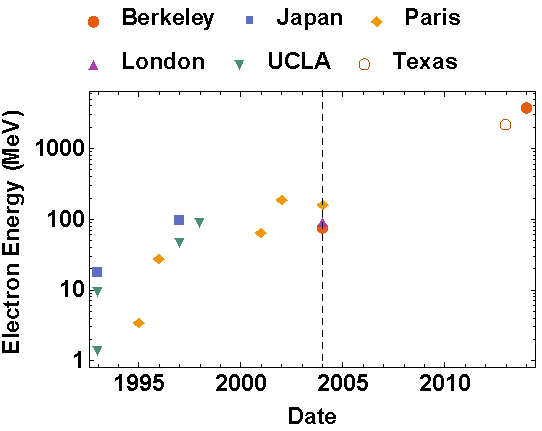
\includegraphics[width=\marginparwidth]{../figures/datfig.pdf}
    \caption{The progress of laser plasma wakefield acceleration by the total
    energy of the electrons. The dashed line shows the advent of
    quasi-monoenergetic electrons, until that point the electron bunches had
    large thermal tails. \em This data was gathered from the web of science
abstract list}
\end{marginfigure}
N
 Plasma accelerator technology then moved in lockstep with improvements in lasers.
 Unfortunately, the electron bunches produced had large thermal distributions.
 
 In 2002, Pushkin predicted the bubble regime, which would solve many of the
 problems historyically faced by LPWA schemes.\cite{}
 In 2004, three papers published simultaneously in Nature\cite{}, demonstrated
 quasi-monoenergetic electron bunches in the bubble regime. Their results were soon extended to
 obtain 1 GeV electron bunches. 
 \todo[inline]{Need to expand this more. Probably should read these papers}

 
 In 2013, a group at UT Austin produced a collumated, quasi-monoenergetic
 electron beam at 2.3 GeV\cite{Wang2013}, and in 2014 the Esarey group at UC
 Berkeley produced a 4 GeV\cite{} beam.

\section{The Physics of Laser-Plasma-Acceleration}
\begin{marginfigure}
    \resizebox{.7\marginparwidth}{!}{
    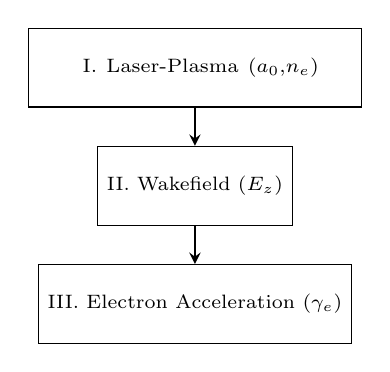
\begin{tikzpicture}[scale =.5,node distance = 1.5cm,auto]
        \node[draw,rectangle,minimum height=1cm,minimum width=2cm,text
        centered, text width = 4 cm,name=input]
        {\footnotesize \setstretch{1} I. Laser-Plasma ($a_0$,$n_e$)\\};
        \node[draw, rectangle, text centered, minimum height=1cm, minimum
        width=2cm, below of=input] (wakefield) {\footnotesize II. Wakefield ($E_z$)};
        \node[draw, rectangle, minimum height=1cm, text centered, minimum
        width=2cm, below of=wakefield] (eaccel) {\footnotesize III. Electron
        Acceleration ($\gamma_e$)};
        \draw  [thick,->,>=stealth] (input) -- (wakefield);
        \draw  [thick,->,>=stealth] (wakefield) -- (eaccel);
    \end{tikzpicture}
}
\caption{\label{fig:flow}The LWFA process: first the intense laser (charaterized
by the normalized field strength ($a_0 = e\vb{A}/m_e c^2$) interacts with the
plasma (characterized by the plasma density ($n_e$) producing a longitudinal
density modulation; this gives rise to a longitudinal electric field ($E_z$);
which will in turn accelerate the electrons to a relativistic energy $\gamma_e$.}
\end{marginfigure}
   
The LPWA process can be divided into three main topics, as shown in Figure
\ref{fig:flow}. This section will review each in turn: first the laser-plasma
interaction will be discussed; then, the wakefield properties will be developed;
and finally, the actual process of electron acceleration will be discussed.

Due to the complicated nature of the theory of LPWA in 3D relativistic fields, we will mainly
discuss these topics in the linear regime, and show the numerical results of
their extension into the 3D relativistic regime.

\subsection{Laser-Plasma Interaction}
As mentioned in Section \ref{sec:history}, it was only the advent of CPA that
allowed lasers to be amplified to the require intensities to see many of the
effects of LPWA. In the non-relativistic regime, the interaction of these laser
pulses with the plasma will be through the Lorentz force\cite{jackson}. As the
mass of the ions in the plasma is many orders of magnitude larger than the
electrons, it is valid to approximate the behaviour of the plasma as a fluid of
mobile electrons against a background of ions.

To first order, the movement of this fluid will be given by the electric force:
$\vb{F} = e\vb{E}$, which will accelerate the electrons in the polarization
plane. This is called the `quiver` momentum\footnote{So named because the electron will
undergo rapid oscillations while its time averaged acceleration will be zero, so it will appear to be quivering}. This quiver momentum will not produce a net acceleration on the 
electrons.

If the Lorentz force law is expanded out to second order, a term will appear that is
proportional to the intensity gradient, known as the ponderomotive force. This can be
thought of as the radiation pressure of the laser pulse, and will act to push
electrons away from the local space of the laser packet. It is this
ponderomotive force that will be directly used to drive the density waves that
all LPWA schemes use. This is analogous to the physical situation of shooting a
cannonball underwater-- it will excite a density wave that co-propogates with
it.

Although tempting to imagine directly accelerating electrons using
the ponderomotive force, it is worth noting that it scales inversely proporitional to gamma: at relativistic speeds it will be small. This is why the density wave is so important.


It is worth noting that modern LWFA schemes operate in the bubble regime, where the laser pulse is so
intense that it completely expels the electrons from its local space.
This regime are too complicated to solve analytically. This means that the 
majority of theoretical work currently being done is by using numerical methods. However, an intuition for the basic
phenomena of LWFA can be developed by looking at simpler systems.

\subsection{Wakefield Dynamics}

As the electron fluid is perturbed by the ponderomotive force, there will be a
large space-charge restoring force that acts upon them. In the simplest,
one-dimensional case, this will give rise to a driven-oscillator type
longitudinal density
modulation that
oscillates at the resonant frequency of the plasma ($\omega_p$). This is
analogous to the ringing sound produced by striking a metal block.

More formally, the equation that will govern the LPWA dynamics is:
\begin{equation}
    \label{eq:fullLPWA}
    \pdv{\vb{p}}{t} +(\vb{v} \cdot \grad)\vb{p} =
            \underbrace{\frac{e}{c}\pdv{A}{t}}_\text{fast time scales} -
            \underbrace{m_ec^2 \grad^2 \bar{a_0}}_\text{slow time scales},
    \end{equation}
In the regime where the normalized field strength is small ($a_0
\ll 1$) this can be linearalized, and are tractable to analytic
techniques. 

More generally, for the relativistic case where ($a_0 /g 1$), there will
non-linear modifications. First, the ponderomotive force generalizes to $a_0
\rightarrow \bar{\gamma} = \qty(1 + \frac{p^2}{m^2c^2} + \frac{a_0^2}{2})^\frac{1}{2}$ Physically, these manifest as steepening phenomena,
where the wave becomes steeper-- very similarily to the process of wavebreaking
of ocean waves.

The resonant frequency of the plasma will give an experimental constraint. As
with all driven-oscillator type systems, to drive the oscillator at resonance,
you need to force it at the natural frequency of the system. We want
high-intensity waves, as their amplitude will ultimately determine the
accelerating field $E_z$. In order to excite resonance then $\tau_\textrm{laser}
\omega_p \approx \pi$. The resonance condition is further illustrated in Figure
\ref{fig:resonance}.

The numerical solutions to Eq. \eqref{eq:fullLPWA} are in Figure \ref{fig:plasmon}.
   \begin{figure}[h!]
       \centering
       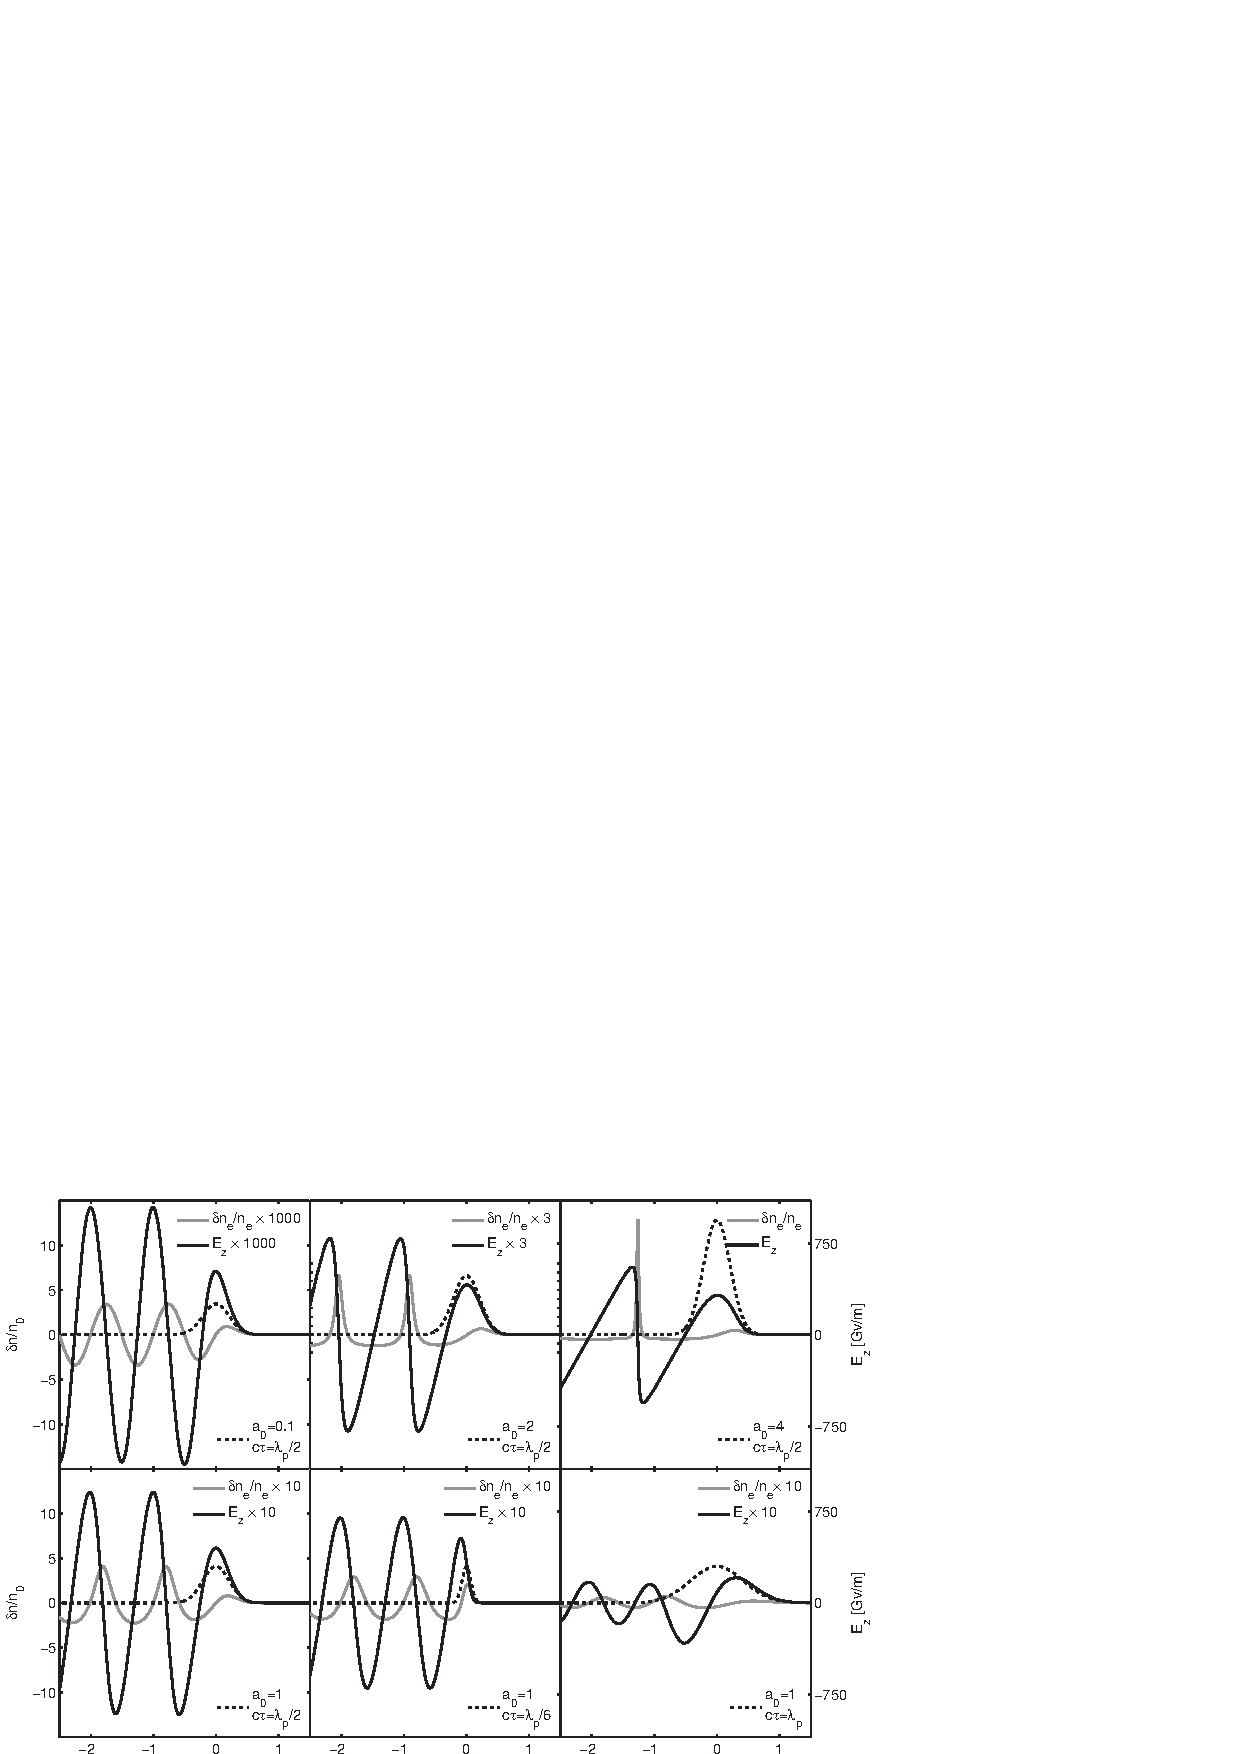
\includegraphics[width = \linewidth]{../figures/densityandewave.pdf}
       \caption{Showing plasmons generated with varying strengths of the peak
       amplitude of the laser pulse.\cite{genothesis}\label{fig:plasmon}
    The laser pulse is the dashed line, the density perturbation is the grey
line, and the longitudinal electric field $E_z$ is the black curve. Different
scenarios are shown: from left to right, the normalized field strength variable
($a_0 = e\vb{E}/m_e c^2$) is varied, and from top to bottom, the duration of
the laser pulse is changed. \em Figure courtesy of Guillaume Genoud, Lund
Univeristy}
   \end{figure}

\pagebreak

   In summary, we have discussed the mechanism of acceleration (longitudinal
   electric field produced by the density wave), and we have discussed how we
   create this mechanism within the plasma (high-intensity laser pushes
   electrons with the ponderomotive force.) Now, we have to discuss how the
   electrons are actually accelerated. Much like water waves, plasmons cannot
   accelerate objects unless two conditions are met\cite{PhysRevLett.113.085001}: the object needs to meet
   some phase-matching requirements, and the plasmon needs to be non-linear. 


   \subsection{Electron Trapping, Injection, and Acceleration}

    In order to be accelerated by the co-propogating electric field created by the
    plasmon, the electrons need to be travelling at some minimum speed. In the
    plasmon frame of reference, what an electron will see is, roughly, an
    ion-sphere. If we confine the electrons motion to 1D, then it can exhibit
    periodic motion about the centre of this sphere. 

    However, for this to work, the electron needs to have some minimum energy.
    Imagining a simple harmonic potential that is moving at some brisk speed $v_b >
    \sqrt{2 V_\mathrm{height of well}/m} $, we can see that an electron at rest will
    not be trapped: transforming to the potential's frame of reference, the
    electron will be moving at a large speed and will have too much energy to be trapped.
    This is quite similar to the case we are describing: however, we now have to
    consider that the electron's motion is going to be relativistic. The
    phase-space trajectories of various electrons are shown in Figure
    \ref{fig:trapping}.
\begin{figure}[h]%
	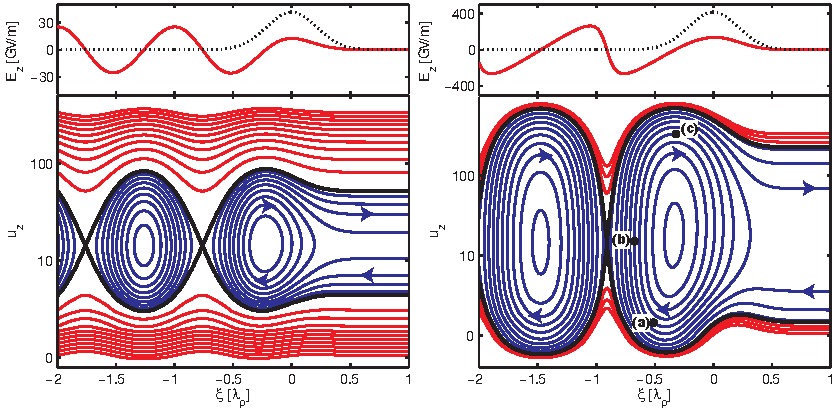
\includegraphics[width=\textwidth]{../figures/trapping.pdf}
    \caption{\label{fig:trapping} The various trajectories of electrons at
    different initial momentum ($u_z= p/m_e c^2$) in the reference frame of the laser
pulse, which is moving at an relativisitc energy $\gamma = 13$ in the lab frame.
For specific initial electron energies the electrons will be trapped and
accelerated by the wakefield. }
\end{figure}

However, much like how the individual water particles do not gain a net
acceleration in ocean waves, in the linear regime the electrons will not gain a
net acceleration.
    For a very specific value of the accelerating electric field the background
    electrons that make up the density flucuations will actually meet the
    requirements to be trapped in this way. This gives rise to the phenomena of
    wavebreaking. In contrast to the perhaps more familiar example of water-wave's
    breaking, plasma wavebreaking is not a dispersion related phenomena. It is a
    non-linear effect, where the accelerating field created by the density
    flucuations of electrons in the plasma is strong enough to directly effect the
    density flucuations themselves.

    Wavebreaking is a useful phenomena for LWFA as it creates a larger field that
    can give more energy to the electrons. The phenomelogical differences between a
    linear plasmon and a wavebroken plasmon are show in Figure \ref{fig:plasmon}

    \subsection{Electron Acceleration}
    The plasma bubble will set up a very high \si{\giga \electronvolt \per
    \centi \meter} acceleration field, however what will limit the total energy
    gain is how far the electron can be accelerated for. 
    There are three main lengths involved with accelerating the
    electrons.
    
    The first, $L_\mathrm{Dephasing}$ is analogous to what happens
    when a surfer outruns the wave they are on; no longer being accelerated,
    they slow down as their energy is dissapated to the waves. Similarly, electrons
    can outrun the plasma bubble. 

    The second, $L_\mathrm{Pulse Depletion}$, occurs because the interaction
    with of the laser-plasma will dissipate the energy of the initial laser
    pulse. The energy in the initial laser will be transfered to the plasma
    wake, where it will ultimately be disappaited as heat. 

    The third length, $L_\mathrm{Diffraction}$ is the most important, as it is
    the limiting length scale. This length scale is due to the inherent
    diffraction of lasers. In order to achieve the intense energies neccesary
    for the bubble regime, the lasers need to be focused down to a specific spot
    size. As soon as the minimum spot size is reached, the laser will begin to
    diffract, the length scale where the laser is approximately the spot size is
    the Rayleigh length. In a plasma this becomes more complicated, as the
    plasma can and will act like a lens. This leads to a feedback effect, where
    the intense laser pulse will change the plasma density, which in turn
    changes the intense laser pulse, and so on. The majority of effort in current wakefield accelerator  programs is to overcome this issue.

    In Figure \ref{fig:energy}, we can see the length scales multiplied by the
    accelerating electric field-- giving the total energy possible if an
    electron was accelerated over that distance. Clearly, the limiting length
    scale is diffraction.
    \begin{marginfigure}
        \begin{subfigure}[t]{\marginparwidth}
            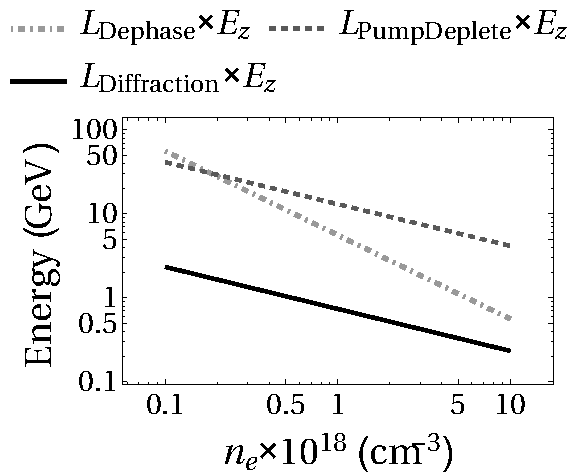
\includegraphics[width=\linewidth]{../figures/energy.pdf}
        \end{subfigure}
        \caption{The three length scales involved with accelerating electrons:
        $L_\mathrm{Dephase}$ where the electron outruns the wave, self-limiting
    the total energy gained; $L_\mathrm{Pump Depletion}$ where the incident
energy in the laser pulse is completely transfered to the wakefield, and the
laser can no longer sustain the bubble regime; and $L_\mathrm{Diffraction}$ the
inherent diffraction of the laser pulse. All lengths are scaled by an
accelerating field using parameters from the Texas
experiment\cite{Wang2013}, to show the total possible energy an electron
could gain.\label{fig:energy}}
    \end{marginfigure}

    There are several strategies for extending the length of the laser-plasma
    interaction: two that we will mention are relativistic self-focusing, and
    external plasma-waveguide solutions. These are the two main solutions
    currently being pursued by the UT Texas group and the Berkeley group,
    respectively.

\section{Experimental Set-Up and State-of-the-Art}
In this review, we will focus on the experimental efforts of two groups, UT
Austin Texas, and University of California Berkeley. Although there are many
more groups doing interesting work in the field of LWFA, these two groups are
the main ones actively pursuing the goal of high-energy electron
accleration.

The Texas group uses very high-intensity laser pulses and exploits the
phenomena of relativistic self-guiding to cancel out the inherent diffraction
of the laser. The Berkeley group uses low-intensity laser pulses and plasma waveguide channels to overcome the diffraction issue. A more in depth review of
each group and method is presented below.

\subsection{Texas: Relativistic Focusing}

In 2013, the Texas group reported a collumated beam of \SI{2}{\giga
\electronvolt}, which blew current records out of the
water\cite{Wang2013}.

Their approach used the new petawatt laser facility at UT Austin. The large
amplitudes that the laser was capable of generating placed them firmly in the
relativisitic self-guiding regime.

\subsubsection{Relativistic Self-Guiding}
The group velocity of the laser pulse will be set by the index of refraction of
the medium, which in turn is $eta = v_g/c = c^{-1}\dv{w}{k}$.  The dispersion
relation for a plasma is shown in Figure \ref{fig:disperion}. Thus,
\begin{equation}
    \label{eq:index}
    eta = \qty(1-\frac{\omega_p^2}{\omega^2})^{1/2}.
\end{equation}

If $eta$ has a density distribution where it is larger on the optical axis, then
a guiding plasma lens will be formed that can counteract the effects of
diffraction. As we will discuss below, one can use relativistic effects to
achieve this. 
\begin{marginfigure}
    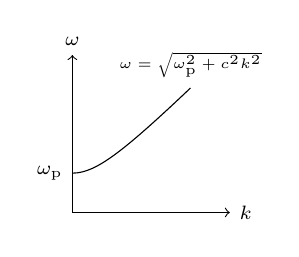
\begin{tikzpicture}[domain=0:4,scale=.5]
        \draw[->] (0,0) -- (4,0) node[anchor=west,font=\footnotesize] {$k$};
        \draw[->] (0,0) -- (0,4) node[anchor=south,font=\footnotesize] {$\omega$};
        \draw (0,1) node[anchor=east,font=\footnotesize] {$\omega_\mathrm{p}$};
        \draw[scale=1, domain = 0:3,smooth,variable=\x,black] plot ({\x},{sqrt(\x*\x+1)})
        node[above,font=\tiny] {$\omega = \sqrt{\omega_\mathrm{p}^2 + c^2 k^2}$};
\end{tikzpicture}
    \caption{\label{fig:dispersion}The plasma dispersion relation. We will be
        dealing with plasmas where $\omega_\mathrm{p}/\omega << 1$, so to
    first order the laser will be dispersionless. }
    \end{marginfigure}

Remembering back to Section \ref{sec:laser}, the first order effect of the
high-intensity laser pulse will make the electrons quiver in the polarization
plane.If the laser is intense enough, the electrons will be quivering
relativistically, and will have maximum energy as they pass through the optical
axis of the pulse. This means that their mass will be a maximum on the optical
axis. This can be roughly seen to change the index of refraction, as:
\begin{equation}
    \label{eq:indexrel}
    \eta(m_e) \rightarrow \eta(\gamma m_e) \approx
1-\frac{\omega_p^2}{2\omega^2}\frac{\delta n(r)}{\gamma}
\end{equation}
where $\delta n(r) $is a density variation, and $gamma$ will be a maximum on
axis.\cite{esarey} This gives rise to the focusing behaviour
discussed above.

This sets a very harsh experimental parameter, as the fields have to be
relativistic enough to be able to counter the effects of diffraction. It can be
shown that this limit is that the power in the field is P(GW) = 17.4
$(\omega/\omega_p)^2$\cite{esarey}.

In reality, the dynamics are much more complicated, and require detailed
numerical simulations, one such example is shown in Figure
\ref{fig:propsim}\cite{Wang2013}. This is partially due to the fact that the
front and back of the waves will not satisfy the relativistic criterion, and
diffract away-- dynamically changing the pulse shape, which can have an effect.
\begin{marginfigure}
	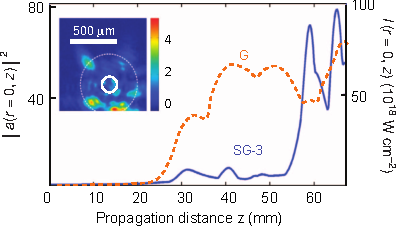
\includegraphics[width=\marginparwidth]{../figures/wakesimulation.pdf}
    \caption{Simulations done by the Texas group using the WAKE
        code showing clear features of self-focusing.\cite{Wang2013} As the
        normalized laser-intensity gets larger, the pulse is
        contracting--concentraing more of its energy over a smaller area.
        Interestingly, the self-focusing exhibits a periodic structure-- going
        through two cycles of diffraction-focusing for the super-gaussian
    pulse.\label{fig:propsim}}
\end{marginfigure}

\subsubsection{Experimental Setup and Results}
Shown in Figure \ref{fig:experTexas} is the experimental setup for Texas. At
its heart, it is a high-intensity laser that is hitting an ionized gas. The
majority of the experiment is the diagnostics, which allow the team to determine
the energy and spread of the electrons.
\begin{figure*}[b!]
	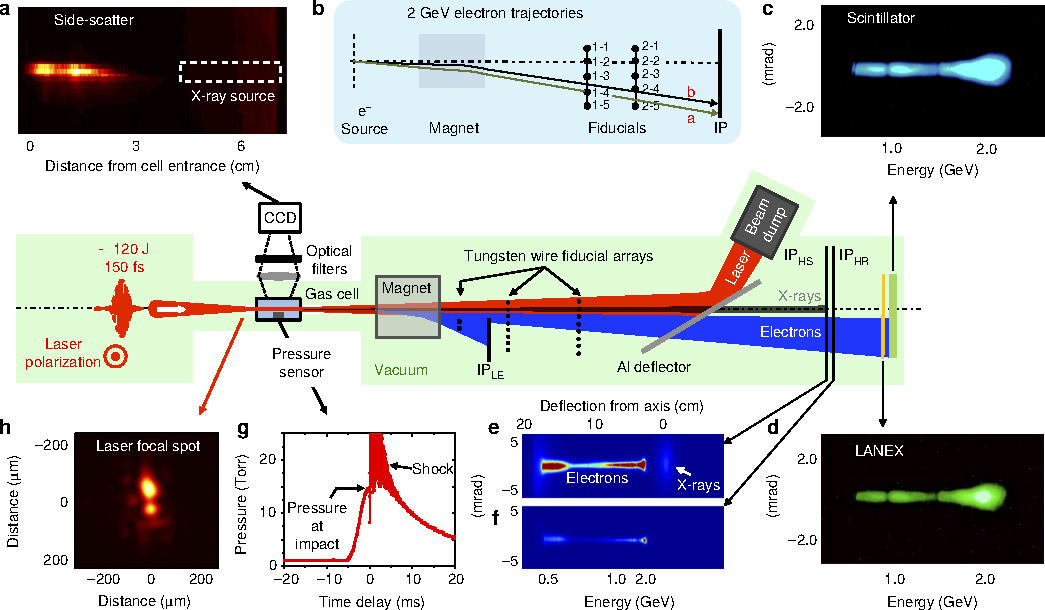
\includegraphics[width=500pt,height=250pt]{../figures/texasexplayout.pdf}
    \caption{The experimental setup of the Texas group.\cite{Wang2013} \em{This
            figure is reproduced from Nat. Commun. Vol. 4, 2013
            \label{fig:experTexas} 
    }}
\end{figure*}

The Texas group is now hard at work trying to find a strategy to increase the
energy of the electrons. Although their initial result is very promising, there
isn't a clear way forward. This is due to the very complicated dynamics of the
highly non-linear laser-plasma interaction that leads to self-focusing. As
shown in Figure \ref{fig:propsim}, the behaviour of the self-focusing is very
dependent on initial conditions (laser intensity, laser pulse shape, etc.). As
no analytic model can fully encompass its behaviour, numerical simulation is
required to understand the self-focusing behaviour required to produce
accleration lengths required for high energy electrons.

Their current work is focused on visualizing and understanding the propogation
of high-intensity laser light through their plasma, and they have developed
several novel techniques.

\todo[inline]{Expand on this-- quickly summarize the visualization thesis. Cite
a few of their more recent papers}

\subsection{Low-Intensity, Quasi-Linear Plasmas with Waveguides}
In 2014, the Berkeley group reported a collumated electron beam with peak
energy of \SI{4.2}{\giga \electronvolt}.

The Berkeley has, for a while now, pursued the strategy of low-intensity laser
pulses that are guided through channels. Their most current results use a
capillary discharge channel. 

The benefits over the Texas strategy is that they gain signifigantly on energy
conversion. Because they don't need to enter into the self-focusing regime,
they can use much less powerful lasers, and compensate by accelerating the
electrons over a larger distance. 
\section{Future Work and Outlook for the Field}
\section{Conclusion}
    \begin{equation}
        \label{eq:wp}
        \omega_\mathrm{p} = \sqrt{\frac{e^2 n_e}{m_e \epsilon_0}}.
    \end{equation}
    Where $m_e$, $n_e$, and $e$ are the mass, density and charge of the electron, respectively.
\bibliography{../rep.bib}
\end{document}

